\NeedsTeXFormat{LaTeX2e}
\documentclass[a4paper,12pt,
headsepline,           % Linie zw. Kopfzeile und Text
oneside,               % einseitig
pointlessnumbers,      % keine Punkte nach den letzten Ziffern in Überschriften
bibtotoc,              % LV im IV
%DIV=15,               % Satzspiegel auf 15er Raster, schmalere Ränder   
%BCOR15mm               % Bindekorrektur
%,draft
]{scrartcl}

\usepackage{amsmath}
\usepackage{amsfonts}
\usepackage{amssymb}
\usepackage{enumitem}
\usepackage[utf8]{inputenc} % this is needed for umlauts
\usepackage[ngerman]{babel} % this is needed for umlauts
\usepackage[T1]{fontenc} 
\usepackage{commath}
\usepackage{xcolor}
\usepackage{booktabs}
\usepackage{float}
\usepackage{tikz-timing}
\usepackage{tikz}
\usepackage{multirow}
\usepackage[final]{pdfpages}
\usepackage{blindtext}
\usepackage[scaled]{helvet}
\usepackage{hyperref}
\usepackage{comment}
\usepackage{mathtools}
\DeclarePairedDelimiter{\ceil}{\lceil}{\rceil}

\usetikzlibrary{calc,shapes.multipart,chains,arrows}

\KOMAoptions{DIV=last} % Neuberechnung Satzspiegel nach Laden von Paket helvet

\usepackage{scrpage2}
\pagestyle{useheadings}

\renewcommand{\familydefault}{\sfdefault} 

\setlength{\parindent}{0pt}   % kein linker Einzug der ersten Absatzzeile
\setlength{\parskip}{1.4ex plus 0.35ex minus 0.3ex} % Absatzabstand, leicht variabel

\newcommand{\fullname}{Gruppe 10}
\newcommand{\titel}{Softwaregrundprojekt Meilenstein 3}
\newcommand{\jahr}{2018}
\newcommand{\dozent}{Florian Ege}
\newcommand{\betreuer}{Stefanos Mytilineos}
\newcommand{\fakultaet}{Ingenieurwissenschaften, Informatik und\\Psychologie}
\newcommand{\institut}{Institut für Softwaretechnik und Programmiersprachen}

\pdfinfo{
    /Author (\fullname)
    /Title (\titel)
    /Producer     (pdfeTex 3.14159-1.30.6-2.2)
    /Keywords ()
}

\hypersetup{
    pdftitle=\titel,
    pdfauthor=\fullname,
    pdfsubject={Softwaregrundprojekt-Abgabe},
    pdfproducer={pdfeTex 3.14159-1.30.6-2.2},
    colorlinks=false,
    pdfborder=0 0 0	% keine Box um die Links!
}

% Trennungsregeln
\hyphenation{Sil-ben-trenn-ung}


\begin{document}
    \thispagestyle{empty}
    \begin{addmargin*}[4mm]{-10mm}

        
\includegraphics[height=1.8cm]{images/unilogo_bild}
        \hfill
        
\includegraphics[height=1.8cm]{images/unilogo_wort}\\[1em]

        {\footnotesize
        %{\bfseries Universität Ulm} \textbar ~89069 Ulm \textbar ~Germany
        \hspace*{115mm}\parbox[t]{35mm}{\bfseries Fakultät für\\
        \fakultaet\\
        \mdseries \institut}\\[2cm]

        \parbox{140mm}{\bfseries \LARGE \titel}\\[2.5em]
        {\footnotesize Softwaregrundprojekt an der Universität Ulm}\\[3em]

        {\footnotesize \bfseries Vorgelegt von:}\\
        {\footnotesize \fullname\\}\\ [1em]
        {\footnotesize \bfseries Dozent:}\\
        {\footnotesize \dozent\\}\\[1em]
        {\footnotesize \bfseries Betreuer:}\\
        {\footnotesize \betreuer}\\ [1em]
        {\footnotesize \jahr}
        }
    \end{addmargin*}
    \pagebreak
    \tableofcontents
    \pagebreak
  
    \section{Schnittstellenarten, Dialoge und Dialogstruktur}
    Der Client stellt die Anwendung dar, mit der ein Nutzer aktiv als Spieler oder auch passiv als Beobachter an einer Partie teilnehmen kann.

\subsubsection{Schnittstellenarten}
Als Benutzerschnittstelle wird eine grafische Benutzeroberfläche verwendet. \\ \textbf{Begründung:} Um das Spiele so intuitiv wie möglich zu gestalten, ist es sinnvoll, dem Nutzer alle für das Spielgeschehen relevanten Informationen und Aktionen grafisch in einer GUI darzustellen. Hinzu kommt, dass neben dem eigentlichen Spiel auch die zugehörigen Funktionen, wie zum Beispiel das Verbinden mit einem Server, benutzerfreundlich und leicht zu bedienen sein sollte. Dies lässt sich am leichtesten durch eine grafische Benutzeroberfläche bewerkstelligen.

\newpage

\subsubsection{Dialoge}
Im Folgenden sind alle Dialoge, die während der Nutzung des Clients benötigt werden, den zugehörigen Anwendungsfällen zugeordnet. 

\begin{figure}[H]
    \centering
    \begin{tabular}{|p{\textwidth/4} p{\textwidth/12} p{\textwidth/16} p{\textwidth/2}|}
        \hline
        \textbf{Name} & \textbf{Typ} & \multicolumn{2}{l|}{\textbf{Abgedeckte Anforderungen}} \\\hline
        Startbildschirm & Dialog & FA60 & Hauptmenü [Ansicht]\\\hline
        Hilfe & Dialog & FA65 & Hilfe [Ansicht]\\
        & & QA18 & Benutzerfreundlichkeit\\\hline
        Hotkey-Liste & Dialog & FA65 & Hilfe [Ansicht]\\
        & & FA68 & Hotkeys\\\hline
        Team ändern & Popup & FA63 & Team-Konfiguration importieren [Ansicht]\\
        & & FA15 & Teams\\
        & & FA54 & Quidditchtem-Konfiguration\\
        & & FA61 & Spiel beitreten [Ansicht]\\\hline
        Beenden & Popup & & \\\hline
        Spielstart fehlgeschlagen & Popup & QA16 & Zuverlässigkeit\\\hline
        Verlassen & Popup & &\\\hline
        Spielsuche & Dialog & FA61 & Spiel beitreten [Ansicht]\\
        & & FA55 & Netzwerkschnittstelle\\\hline
        Spielende & Dialog & FA62 & Spiel Ende [Ansicht]\\
        & & FA49 & Spielende\\\hline
        Beobachten & Dialog & FA66 & Beobachter [Ansicht]\\\hline
        Verbindungsabbruch & Dialog & QA16 & Zuverlässigkeit\\
        & & QA17 & Robustheit\\\hline
        Pause & Dialog & FA69 & Pausieren\\\hline
    \end{tabular}
\end{figure}
\begin{figure}[H]
    \centering
    \begin{tabular}{|p{\textwidth/4} p{\textwidth/12} p{\textwidth/16} p{\textwidth/2}|}
        \hline
        Spiel & Dialog & FA64 & Spiel[Ansicht]\\
        & & FA1 & Spielfeld\\
        & & FA2 & Mittelkreis\\
        & & FA3 & Mittelzelle\\
        & & FA4 & Hüterzone\\
        & & FA5 & Zelle\\
        & & FA6 & Torring\\
        & & FA8 & Punkte erzielen\\
        & & FA10 & Ball\\
        & & FA11 & Quaffel [Ball]\\
        & & FA12 & Klatscher [Ball]\\
        & & FA13 & Goldener Schnatz [Ball]\\
        & & FA14 & Besen\\
        & & FA16 & Spielfiguren\\
        & & FA17 & Jäger\\
        & & FA18 & Treiber\\
        & & FA19 & Hüter\\
        & & FA20 & Sucher\\
        & & FA31 & Fans\\
        & & FA32 & Elfen [Fantyp]\\
        & & FA33 & Kobolde [Fantyp]\\
        & & FA34 & Trolle [Fantyp]\\
        & & FA35 & Niffler [Fantyp]\\
        & & FA36 & Schiedsrichter\\
        & & FA44 & Runde\\
        & & FA46 & Spielerphase\\\hline
    \end{tabular}
\end{figure}

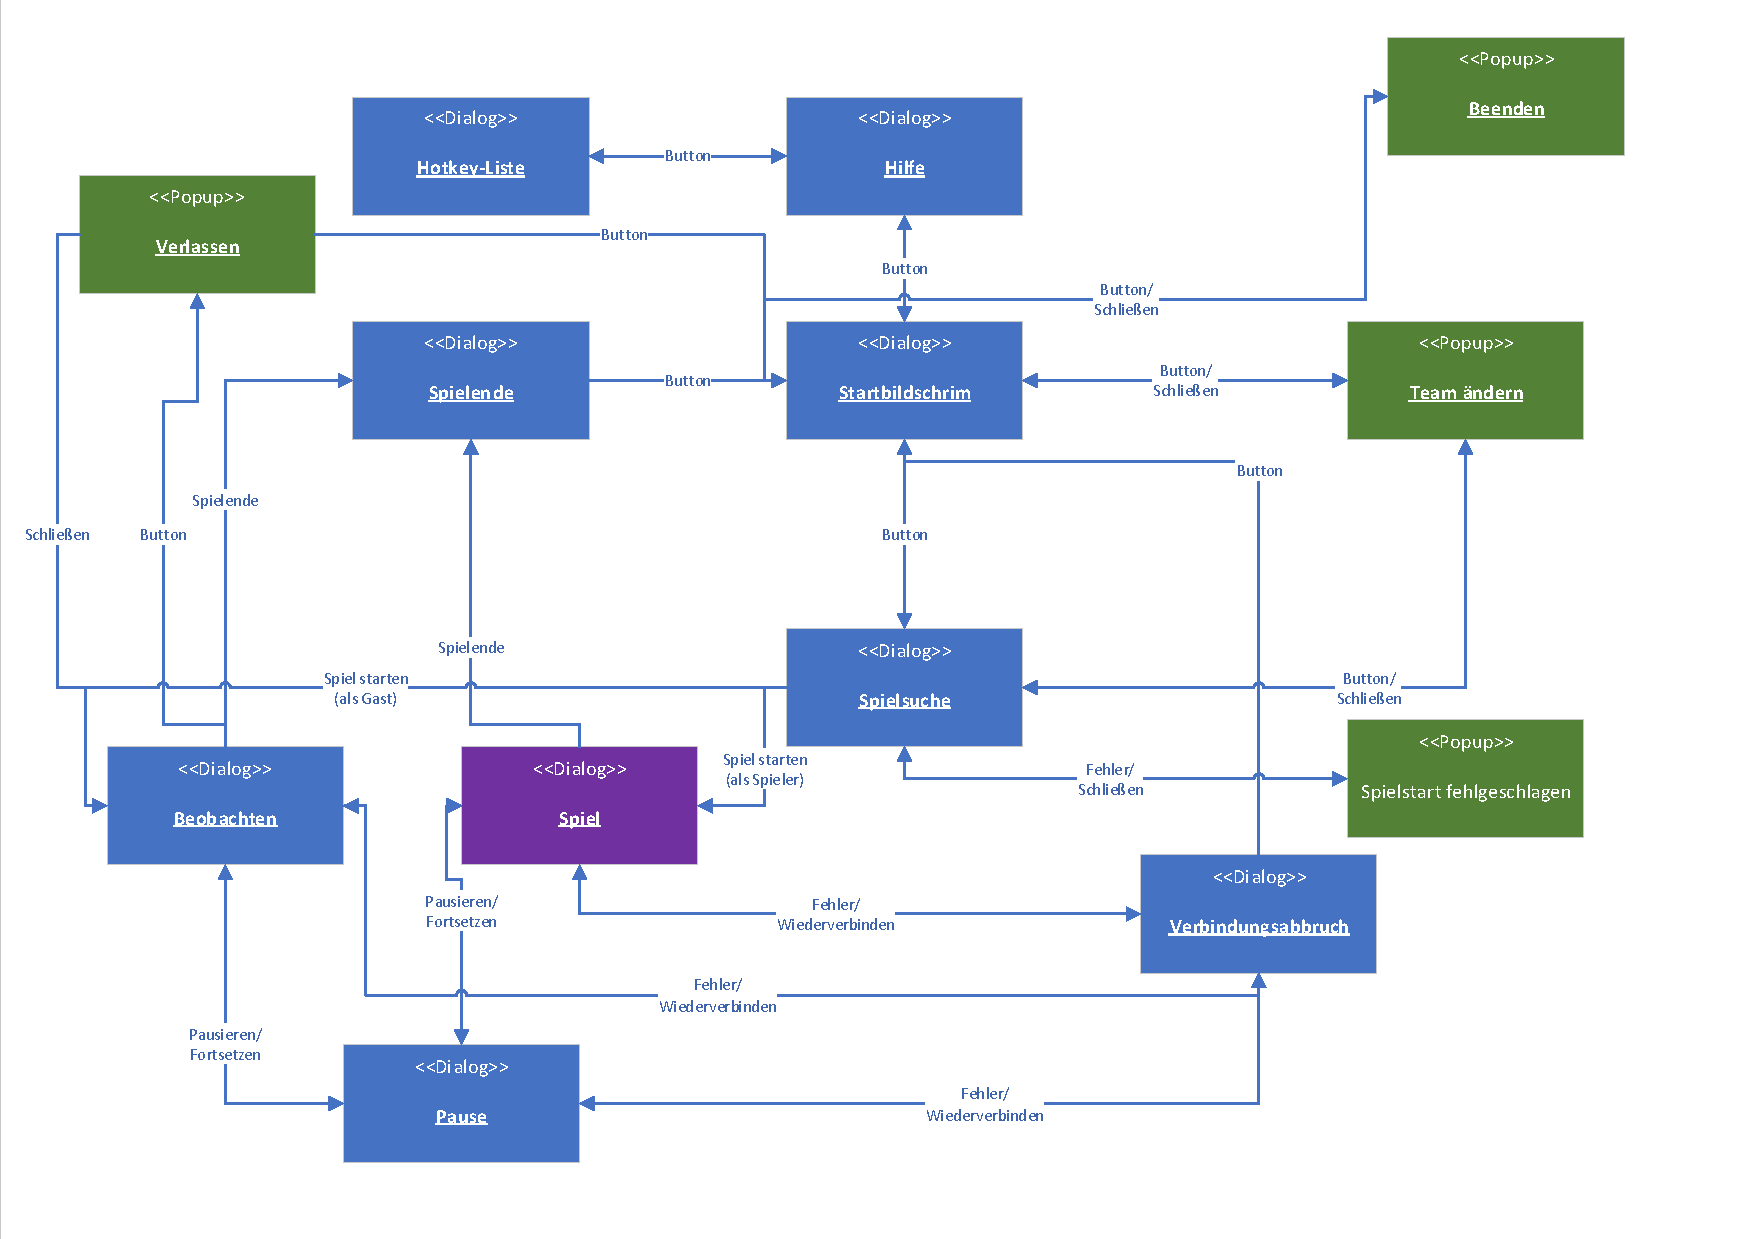
\includepdf[pages=-, scale=0.8, pagecommand={\subsubsection{Dialogstrukturdiagramme}}]{../Meilenstein03/images/Client_Hauptmenue.pdf}

	\section{Grafische Gestaltung und Nutzungskonzept}
    \subsection{Client}

    \subsubsection{Spielansicht für einen Spieler}

    \begin{figure}[H]
        \centering
        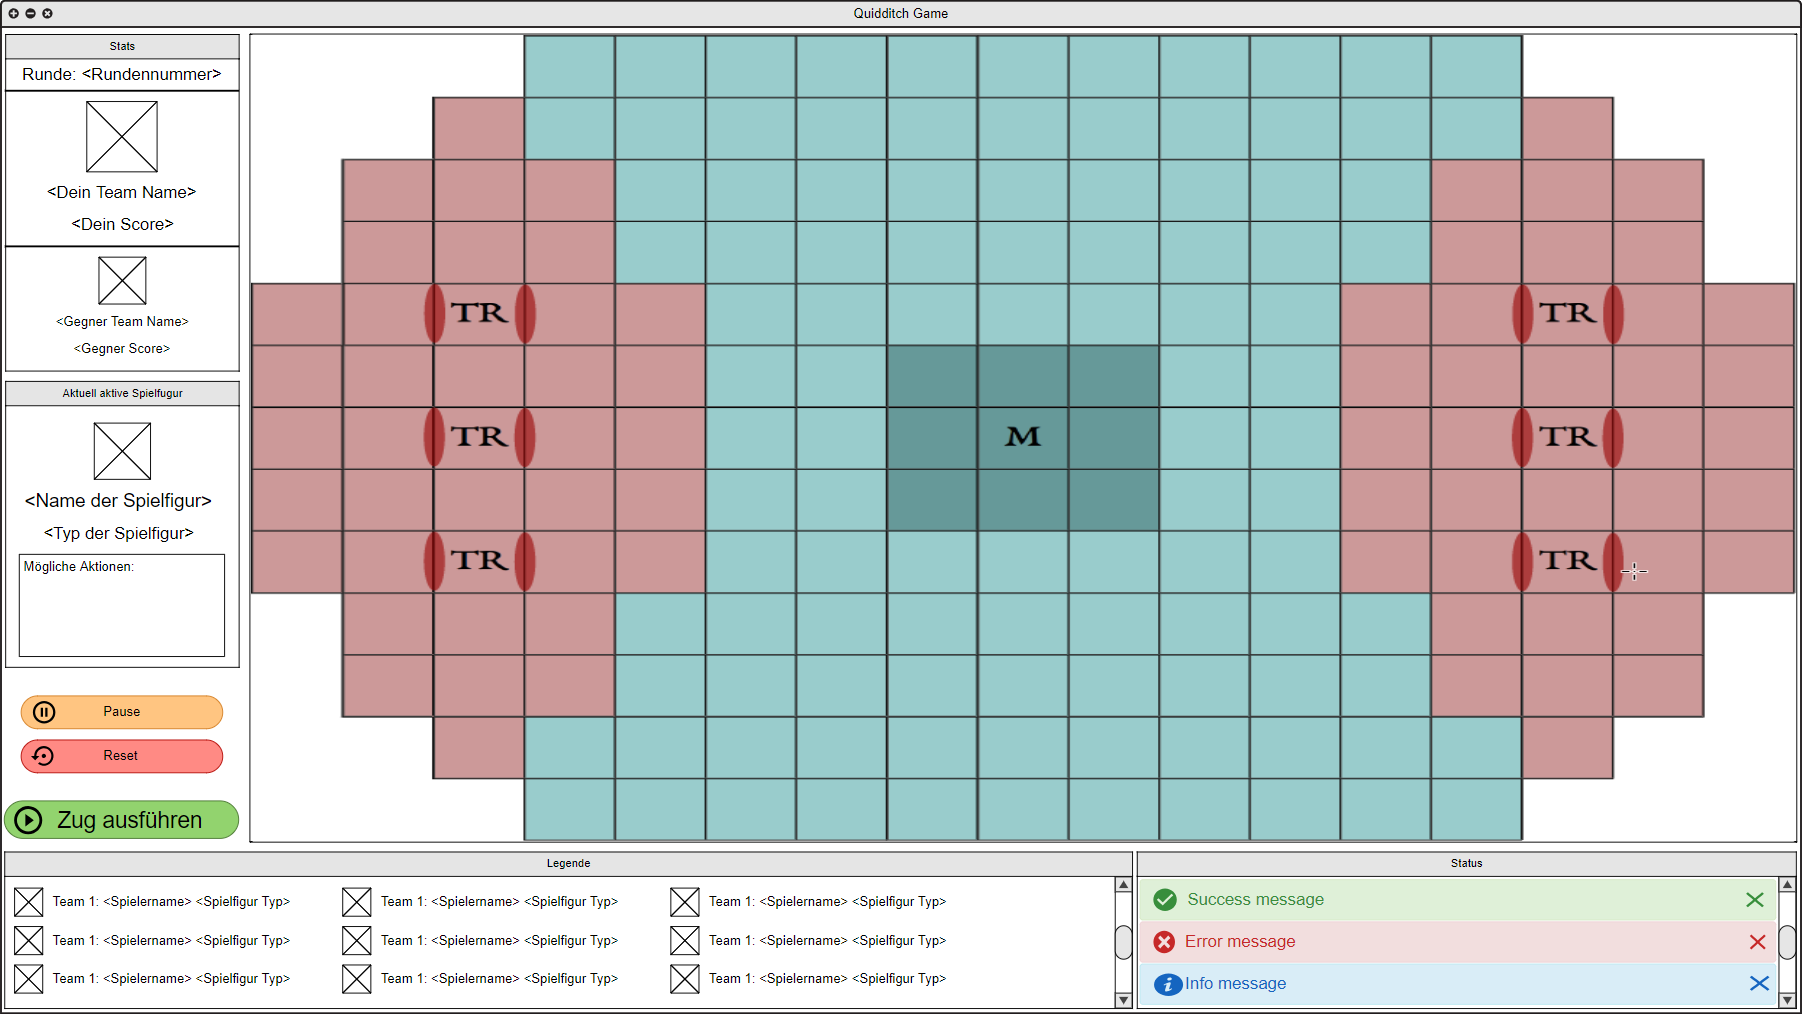
\includegraphics[width=\textwidth]{images/InGamePlayer.PNG}
    \end{figure}

    In der Spielansicht kann ein Spieler das aktuelle Spielgeschehen verfolgen und sein Züge ausführen. Dabei ist die Oberfläche in mehrere Teile unterteilt.\\
    Im \textit{Stats} Bereich werden grundlegende Informationen über die aktuelle Partie und die beiden Teams dargestellt. Das Team, das an oberster Position steht, ist momentan am Zug. Der darunter liegende Bereich ist der \textit{Fan} Bereich. Hier kann der Spieler auswählen, ob und welcher Fan eine Aktion ausführen soll. Darunter befinden sich drei Buttons mit dem entweder das Spiel \textit{pausiert} werden , alle Veränderungen die man in der aktuellen Runde getätigt hat \textit{zurücksetzen} oder seinen Zug endgültig \textit{ausführen} kann. Am unteren Rand der Oberfläche ist eine \textit{Legende} mit einer Übersicht über alle Spielfiguren des eigenen und des gegnerischen Teams zu sehen. Daneben befindet sich ein Feld, in dem Statusmeldungen angezeigt werden können. Beispiele für solche Statusmeldungen sind zum Beispiel eine Benachrichtigung über ein Faul oder über das erfolgreiche Ausführen eines Spielzuges. Der größte Teil der Oberfläche nimmt dass eigentliche Spielfeld ein. Hier werden alle Spielfiguren in den Feldern angezeigt auf denen sie sich gerade befinden. Ist man am Zug und klickt auf einen Spieler, so werden alle Züge, die von der Spielfigur ausgeführt werden können farblich hervor gehoben. Der Spieler kann diese Aktionen dann durch weitere Klicks ausführen und die Prozedur gegebenenfalls für weitere Spielfiguren wiederholen. Ist man nicht am Zug so werden alle Eingabemöglichkeiten, mit Ausnahme des \textit{Pause} Buttons deaktiviert.
    

    \subsubsection{Spielansicht für einen Beobachter}
        
    \begin{figure}[H]
        \centering
        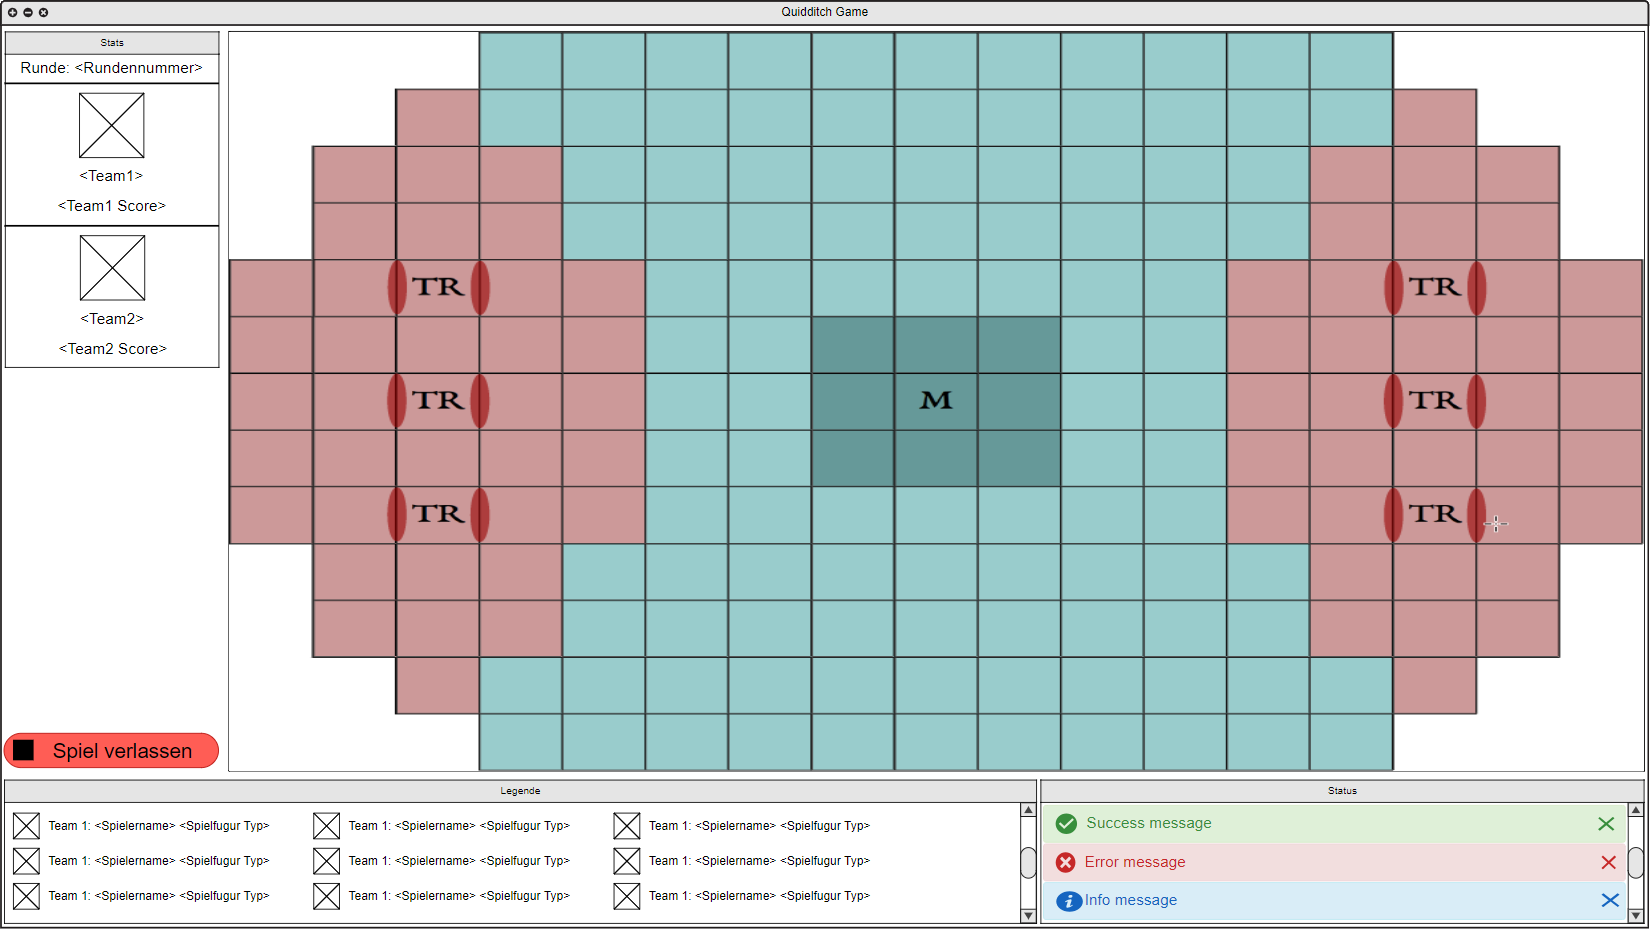
\includegraphics[width=\textwidth]{images/InGameObserver.PNG}
    \end{figure}

    In der Spielansicht kann ein Beobachter eine Partie wischen zwei anderen Gegnern passiv verfolgen. Die Oberfläche ist im wesentlichen gleich aufgebaut wie die Oberfläche, die die Spieler sehen. Jedoch sind beim Beobachter alle Felder die zur Eingabe dienen deaktiviert und teilweise ausgeblendet. Die einzige Interaktion, welche durch einen Button ermöglicht wird ist das vorzeitige \textit{verlassen} einer Partie.
    
    \subsubsection{Startbildschirm}
\begin{figure}[H]
	\centering
	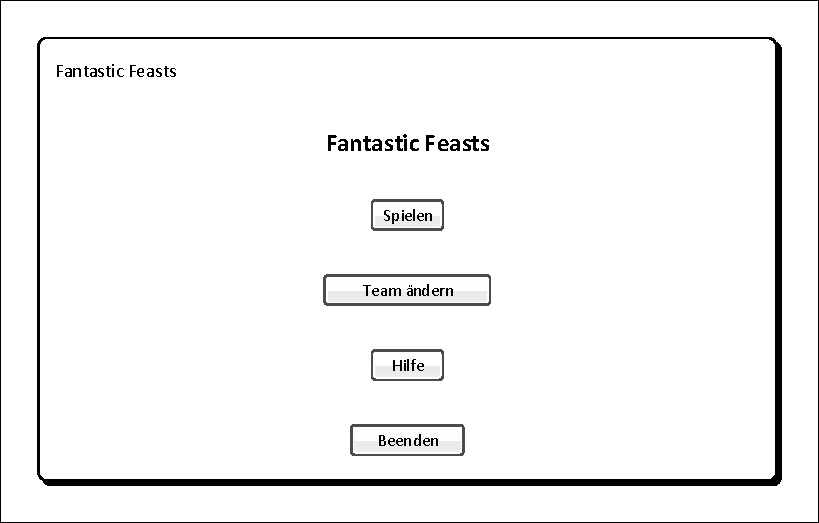
\includegraphics[scale=0.8]{images/Startbildschirm.pdf}
\end{figure}

Dieser Dialog erscheint nach Start der Anwendung. Der \glqq{}Spielen\grqq{}-Button öffnet den Spielsuche-Dialog. Der \glqq{}Team ändern\grqq{}-Button öffnet das \glqq{}Team ändern\grqq{}-Popup. Der \glqq{}Hilfe\grqq{}-Button öffnet den Hilfe-Dialog. Der \glqq{}Beenden\grqq{}-Button öffnet ein Bestätigungs-Popup und beendet bei positiver Antwort die Anwendung.

\subsubsection{Spielsuche}
\begin{figure}[H]
	\centering
	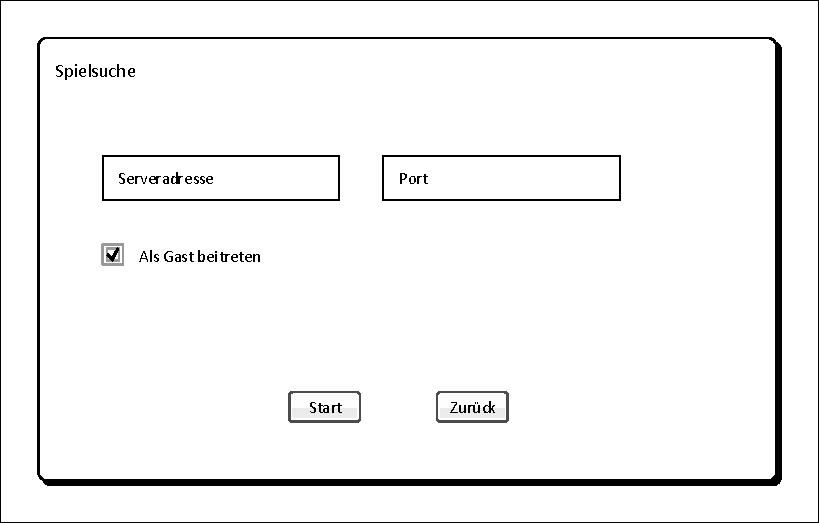
\includegraphics[scale=0.8]{images/Spielsuche.pdf}
\end{figure}

Der Benutzer gibt zuerst die Adresse und den Port des Spielservers und, mit dem er sich verbinden möchte. Wenn er die Partie beobachten will, wählt er \glqq{}Als Gast beitreten\grqq{} aus. Drückt er anschließend auf den \glqq{}Start\grqq{}-Button, versucht sich der Client mit dem angegebene Server zu verbinden. Mit dem \glqq{}Zurück\grqq{}-Button kann man zurück auf den Startbildschirm gelangen.
	
\subsubsection{Hilfe}
\begin{figure}[H]
	\centering
	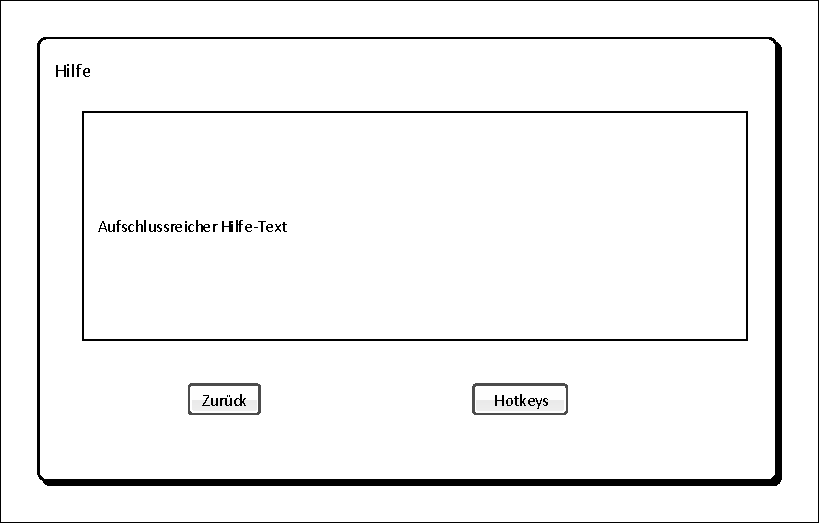
\includegraphics[scale=0.8]{images/Hilfe.pdf}
\end{figure}

In einem großen Textfeld, gegebenenfalls mit Scrollbar, wird ein Hilfetext angezeigt. Der \glqq{}Zurück\grqq{}-Button öffnet den Startbildschirm, der \glqq{}Hotkey\grqq{}-Button den Hotkey-Dialog.

\subsubsection{Hotkeys}
\begin{figure}[H]
	\centering
	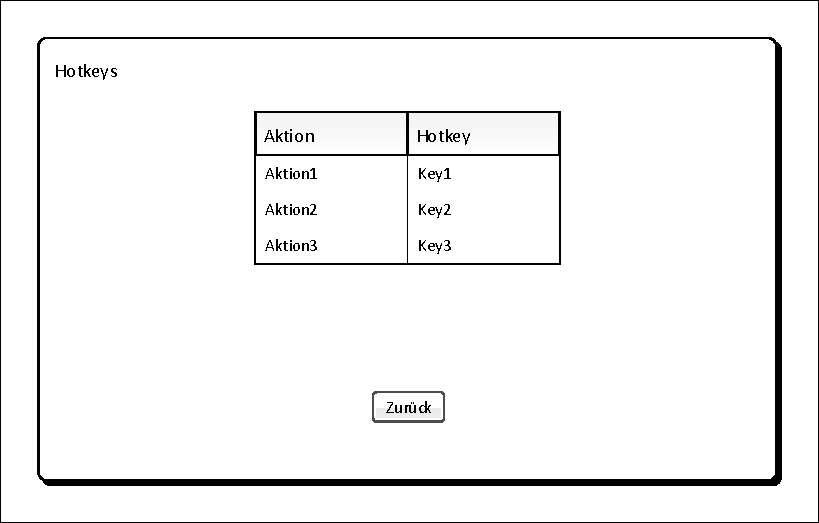
\includegraphics[scale=0.8]{images/Hotkeys.pdf}
\end{figure}

Hier werden alle verfügbaren Hotkeys in Tabellenform aufgelistet. Der \glqq{}Zurück\grqq{}-Button öffnet den Hilfe-Dialog.

\subsubsection{Team ändern}
\begin{figure}[H]
	\centering
	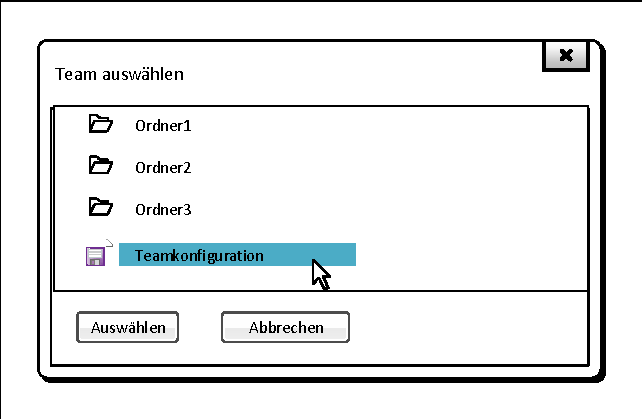
\includegraphics[scale=0.8]{images/Teamauswahl_Popup.pdf}
\end{figure}

In diesem Popup kann der Benutzer durch sein Dateisystem navigieren und eine JSON-Datei auswählen. Hat er eine gültige Datei ausgewählt und betätigt den \glqq{}Auswählen\grqq{}-Button, wird das Popup geschlossen und die Team-Konfiguration für das Spiel verwendet. Der \glqq{}Abbrechen\grqq{}-Button schließt das Popup und es werden keine Änderungen vorgenommen.

\subsubsection{Bestätigungsaufforderung}
\begin{figure}[H]
	\centering
	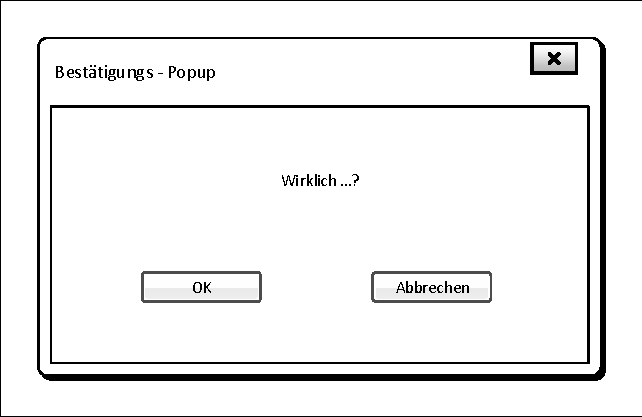
\includegraphics[scale=0.8]{images/OK_Popup.pdf}
\end{figure}

Dieser Aufbau wird für die Popups \glqq{}Beenden\grqq{} und \glqq{}Verlassen\grqq{} verwendet. Der \glqq{}Abbrechen\grqq{}-Button schließt das Popup und der Benutzer gelangt zurück in den Dialog, in dem er vor Öffnen des Popups war. Der "OK"-Button führt dazu, dass eine Aktion ausgeführt wird.

\subsubsection{Fehler}
\begin{figure}[H]
	\centering
	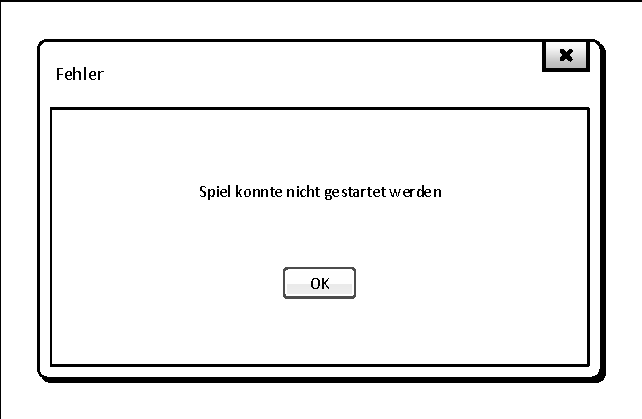
\includegraphics[scale=0.8]{images/Fehler_Popup.pdf}
\end{figure}

Dieser Aufbau wird für das Popup \glqq{}Spielstart fehlgeschlagen\grqq{} verwendet. Der angezeigt Text richtet sich nach dem aufgetretenen Fehler. Der \glqq{}OK\grqq{}-Button schließt das Popup.

\subsubsection{Pause}
\begin{figure}[H]
	\centering
	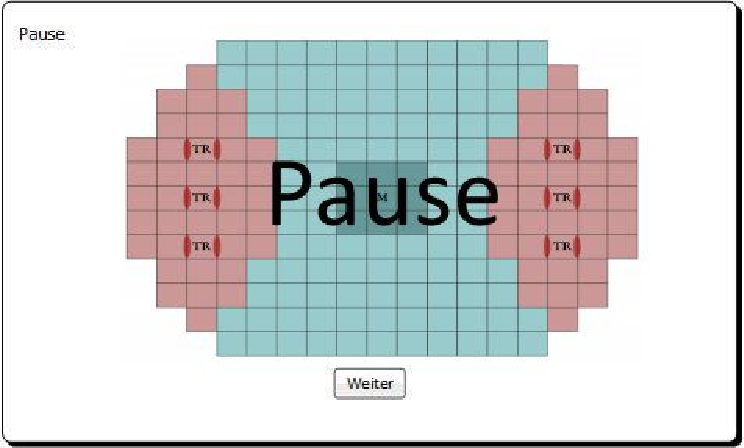
\includegraphics[scale=0.8]{images/Pause.pdf}
\end{figure}

Wird angezeigt, wenn das Spiel von einem Spieler pausiert wird. Der \glqq{}Weiter\grqq{}-Button setzt die Partie fort und kann nicht von einem Gast betätigt werden.

\subsubsection{Verbindungsabbruch}
\begin{figure}[H]
	\centering
	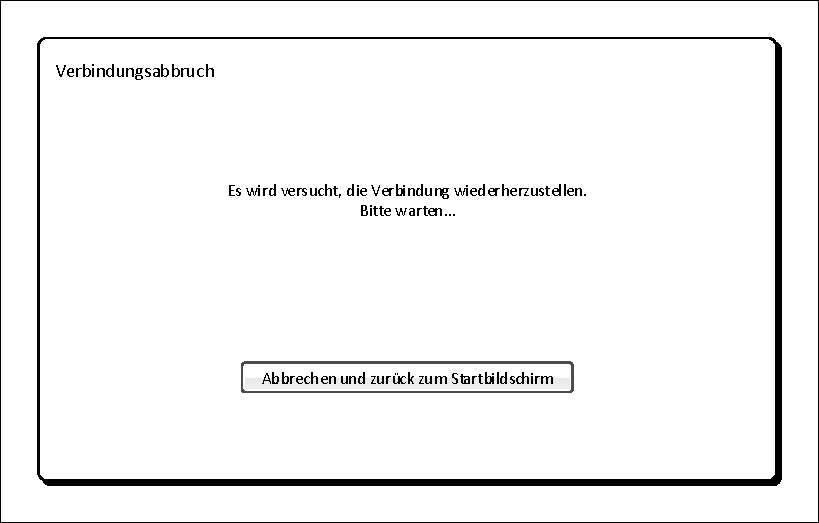
\includegraphics[scale=0.8]{images/Verbindungsabbruch.pdf}
\end{figure}

Im Falle eines Verbindungsabbruchs zwischen Client und Server wird dieser Dialog angezeigt. Wird die Verbindung wiederhergestellt, gelangt der Benutzer automatisch wieder zurück in den vorherigen Dialog. Alternativ kann er durch betätigen des Buttons zum Startbildschirm gelangen. Ist er ein Spieler, kann er die Partie nicht weiterführen und sein Gegner gewinnt nach Ablauf einer Zeitdauer die Partie.

\subsubsection{Spielende}
\begin{figure}[H]
	\centering
	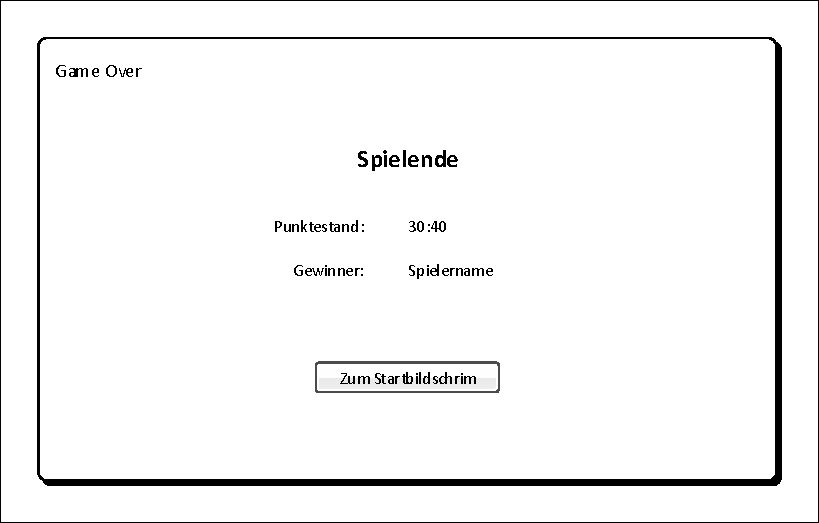
\includegraphics[scale=0.8]{images/Spielende.pdf}
\end{figure}

Bei Spielende wird dieser Dialog geöffnet. Hier werden der Punktestand bei Spielende und der Name des Gewinners angezeigt. Der Button öffnet den Startbildschirm-Dialog.
	
    
    \subsection{Server}
    %TODO: Dialogstruktur Server
    \subsection{Team-Editor}
    %TODO Dialogstruktur Editor
    \subsection{KI-Client}
    Diese Komponente simuliert einen Menschlichen Gegner, der sich wie ein normaler Client bei einem Spielserver anmeldet und dann autonom seine Spielentscheidungen trifft.

\subsubsection{Schnittstellenarten}
Es besteht kein Grund, für diese Komponente eine grafische Oberfläche bereitzustellen, da die Anwendung zur Laufzeit keine Eingabe von einem menschlichen Benutzer erwartet und eine Partie mittels des Clients verfolgt werden kann. \\
Für eine Kommandozeilenanwendung ist es einfacher, Plattformunabhängigkeit sicherzustellen. Außerdem wird es damit problemlos möglich, den KI-Client aus einem anderen Programm zu starten. Beispielsweise kann dem Client eine Funktion hinzugefügt werden, gegen die KI zu spielen, ohne dass der Benutzer den KI-Client extern starten muss.\\

\subsubsection{Dialoge}
Im Folgenden werden die Anforderungen an den KI-Client einem CLI-Dialog zugeordnet.

\begin{figure}[H]
    \centering
    \begin{tabular}{| l l l p{4cm} |}
    \hline
    \textbf{Name} & \textbf{Typ} & \multicolumn{2}{l|}{\textbf{Abgedeckte Anwendungsfälle}} \\\hline
    Init & CLI Befehl mit Params & FA73 - FA75 & Schwierigkeit, Server- und Team-Konfiguration einstellen.\\\hline
	InitFailure & Response & FA73 - FA75 & Feedback.\\\hline
    WaitingForGame & Response & FA55 & Netzwerkschnittstelle, allgemeine Kommunikation.\\\hline
    Playing & Response & allgemein & Feedback.\\\hline
    AttemptingReconnect & Response & FA55 & Netzwerkschnittstelle, allgemeine Kommunikation.\\\hline
    ConnectionLost & Response & FA55 & Netzwerkschnittstelle, allgemeine Kommunikation.\\\hline
    \end{tabular}
\end{figure}

\subsubsection{Dialogstruktur}  
\textbf{Init:} Der KI-Client wird über die Kommandozeile gestartet. Serverkonfiguration, Team-Konfiguration, die maximale Anzahl an Reconnect-Versuchen und der Schwierigkeitsgrad werden beim Start der Anwendung mittels Kommandozeilenparametern gehandhabt. Der Server, mit dem sich der KI-Client verbinden soll wird als Argument übergeben. Die Team-Konfiguration und der Schwierigkeitsgrad können mittels Optionen verändert werden und nehmen ansonsten einen Standardwert an.\\
\textbf{InitFailure:} Wird eine ungültige Option angegeben, ist der Server nicht erreichbar oder wurde eine ungültige Team-Konfigurationsdatei geladen, so erscheint eine Fehlermeldung mit entsprechenden Hinweisen.\\
\textbf{WaitingForGame:} War die Initialisierung erfolgreich und der KI-Client konnte sich mit dem Server verbinden, so erscheint eine Nachricht, die darauf hinweist, dass noch auf den Beginn der Partie gewartet wird.\\
\textbf{Playing:} Während einer laufenden Partie wird ein Hinweis angezeigt.\\
\textbf{AttemptingReconnect:} Bei einem Verbindungsabbruch zeigt der KI-Client eine Meldung an und versucht automatisch, die Verbindung wiederherzustellen.\\
\textbf{ConnectionLost:} Konnte sich der KI-Client nicht innerhalb der angegebenen Anzahl von Versuchen erneut mit dem Server verbinden, so erscheint eine Fehlermeldung und das Programm beendet sich.\\
Der KI-Client beendet sich außerdem nach Abschluss einer Partie durch ein reguläres Spielende. 

\subsubsection{Zulässige Optionen:}
\begin{figure}[H]
    \centering
    \begin{tabular}{|p{2cm}|p{12cm} |}
        \hline
        Flag & Erklärung \\\hline
        -s & Legt den Schwierigkeitsgrad fest.\\
        & Akzeptiert eine ganze Zahl zwischen 0 und 2, wobei 0 für einfach,\\
        & 1 für mittelschwer und 2 für schwer steht.\\
        & Bei einer ungültigen Eingabe wird eine Fehlermeldung ausgegeben.\\\hline
        -t & Legt die Team-Konfiguration fest.\\
        & Akzeptiert einen String als Pfad zu einer JSON-Datei.\\
        & Existiert der angegebene Pfad nicht oder ist die Datei keine gültige Konfigurationsdatei,\\
        & wird eine entsprechende Fehlermeldung ausgegeben.\\\hline
		-r & Reconnects: Spezifiziert, wie oft der KI-Client versucht, die Verbindung nach einem Verbindungsabbruch 
		wiederherzustellen. Standardwert ist 5.\\\hline
        -{}-help & Zeigt eine Liste möglicher Optionen an.\\\hline
    \end{tabular}
\end{figure}

\end{document}
